% !TeX spellcheck = de_DE
%!TEX root = ../../Main.tex
\graphicspath{{Chapters/BluetoothModul/}}
%-------------------------------------------------------------------------------


\subsection{Bluetooth modul}

Bluetooth-modulet der bliver brugt i BA-TA systemet er af typen HC-05. Denne type-version understøtter nemlig mulighed for at tage rollen som både Master/Slave i et Bluetooth Master/Slave forhold imellem to parrende Bluetooth-enheden. Bluetooth modulet er sammensat med et breakout- board i bunden af modulet, hvilket giver nem adgang til de brugbare pins på selve Bluetooth-modulet, hvilket også kan ses på figur \ref{fig:bluetooth_modul}

\begin{figure}[H]
	\centering
	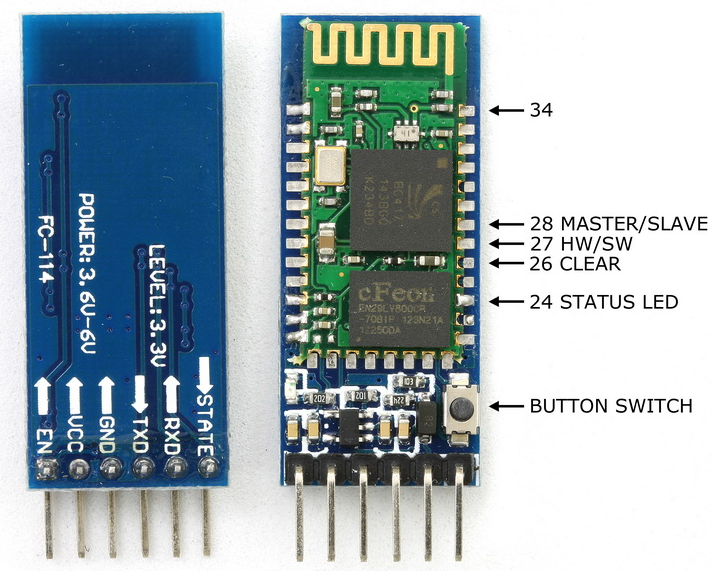
\includegraphics[width = 200 pt]{Img/modul.PNG}
	\caption{Bluetooth modulet: HC-05 GW-040.}
	\label{fig:bluetooth_modul}
\end{figure}

\subsection{Protokol}
Der kommunikeres til systemets Bluetooth-modul igennem en UART-forbindelse. Gruppens implementerede UART-driver på Arduino’en gør det muligt, at Arduinoen og Bluetooth-modulet kan kommunikere sammen vha. AT-kommandoer. 
AT-kommandoerne (Attention-commands) som Bluetooth-modulet understøtter kan bruges til generel opsætning af modulet, sætte Master/Slave roller, scanne for nærtliggende Bluetooth-enheder, samt at spørge om navn på fundne Bluetooth-enheders adresser. AT-kommandoerne er en general standard som bruges til at sende instruktioner til et modul og dermed er de opbygget på samme måde for hvert modul der bruger dem. På en etableret UART forbindelse vil man kunne sende en ”AT+kommando” til modulet, hvorefter modulet vil udføre kommandoen, og evt sende et svar tilbage, samt et OK, hvilket indikerer at beskeder var succesfuldt modtaget af modulet. Det samme er gældende for HC-05 Bluetooth modulet som indgår i BA-TA systemet.
Eksempler på brugte AT-kommandoer til Bluetooth-modulet i BA-TA:

\begin{itemize}
	\item ”AT+INIT” – Initialisering af Bluetooth-modulets Bluetooth SPP profil
	\item “AT+INQM,0,5,4” – Sætter scanner parameter. I dette tilfælde at der maksimum skal findes 5 Bluetooth enheder og at timeout på en scanning af Bluetooth enheder er 4*1.28 sekunder.
	\item ”AT+RNAME?<indsæt,Adresse,Her>” – Bluetooth-modulet spørger om navnet på adressen til den respektive indsætte adresse.
\end{itemize}

En succesfuld AT-kommando vil altid få Bluetooth-modulet til at returnere et OK. Såfremt der eksempelvis bliver spurgt om et navn på en respektiv Bluetooth-enheds adresse, så vil Bluetooth-modulet også returnere den fundne Bluetooth-enheds navn og et OK til sidst. 

\begin{figure}[H]
	\centering
	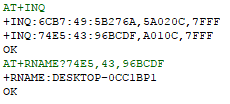
\includegraphics[width = 200 pt]{Img/uart_eksempel.PNG}
	\caption{Kommunikationseksempel med AT-kommandoer ved brug af en UART forbindelse til Bluetooth modulet.}
	\label{fig:UART_eksempel}
\end{figure}

På ovenstående figur,  \ref{fig:UART_eksempel}, kan vi se et eksempel på kommunikation vha. en UART forbindelse til Bluetooth modulet. I eksemplet bliver der sendt et "AT+INQ" til Bluetooth-modulet. Denne besked betyder inquiry, og derfor går Bluetooth modulet straks igang med at undersøge hvilke nærtliggende Bluetooth enheder den kan finde. Herefter svarer den tilbage med et "+INQ:<AdressePåFundetEnhed>" hver gang den har fundet en ny enhed. Dette forsætter den med indtil den når sit maks antal devices eller timeout grænse, som er bestemt af kommandoen "AT+INQM". Når timeout eller maks antal enheder er nået returnerer Bluetooth modulet også et OK for at indikere at den er færdig. Herefter er den også klar igen til at modtage nye beskeder.

\subsection{Implementering}

Da AT-kommandoerne og retur-beskederne er opbygget med samme struktur, har gruppen med fordel taget brug af dette til, at kunne udvikle en Bluetooth-kommunikations-driver, som netop udnytter denne gentagende og genkendelige proces. 

\begin{figure}[H]
	\centering
	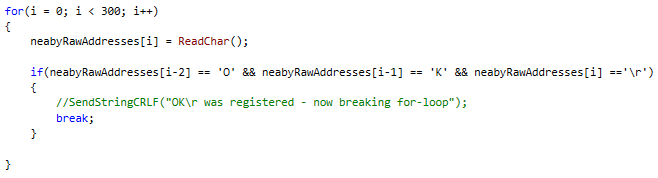
\includegraphics[width = 400 pt]{Img/OK_registrered.PNG}
	\caption{Registrering af det returnede "OK" fra Bluetooth modulet}
	\label{fig:OK_registrered}
\end{figure}

På figur \ref{fig:OK_registrered} kan vi se et eksempel på, hvordan gruppen har udnyttet at der altid vil blive sendt et OK retur til sidst, når Bluetooth modulet indikerer at den er færdig med den instruktionen/kommandoen som den har modtaget forinden. I eksemplet fra figuren benytter gruppen sig af dette til at tjekke hvornår Bluetooth modulet har sendt alt information om Bluetooth enheders adresser, som den har registreret ved sit "AT+INQ".

\begin{figure}[H]
	\centering
	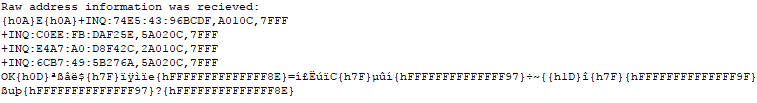
\includegraphics[width = 500 pt]{Img/raw_address.PNG}
	\caption{Al rå adresse information modtaget fra Bluetooth modulet}
	\label{fig:raw_address}
\end{figure}

Herefter kan der analyseres på det char array som alt adresse information for alle fundne enheder ligger i. Formålet med dette er at få skilt informationen ad således vi tage separere de forskellige adresser fra hinanden. Dette skyldes at dataen i det pågældende char array højst sandsynligt er loaded med flere adresser, som det eksempelvis kan ses på figur \ref{fig:raw_address}

Næste skridt er hermed at skille alt den information vi får udover MAC-adressen til de bestemte enheder. Dette gøres ved brug af "delimeter" princippet. Delimeter princippet kan bruges i dette tilfælde, da alle modtagede adresser i char array'et er sammensat og seperaret fra hinanden på en kontinuerlig måde. Hver MAC-adresse starter efter "+INQ:, de 3 dele af MAC adressen er separeret af ":" og MAC-adressen slutter ved et ",". Dette kan også ses på figur \ref{fig:raw_address}.


\begin{figure}[H]
	\centering
	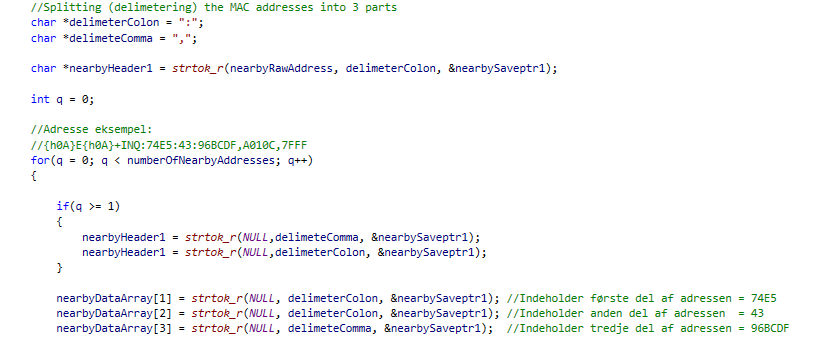
\includegraphics[width = 500 pt]{Img/delimetering.PNG}
	\caption{Brug af "delimeter"\-princippet ved brug af strtok\_r funktionen}
	\label{fig:delimeter}
\end{figure}

På ovenstående figur, \ref{fig:delimeter}, kan vi se det "delimeter"-princippet som er taget i brug for at kunne skære alt andet end de 3 dele af adressen (i dette tilfælde, 74E5, 43 og 96BCDF).

Herefter skal addressen nemlig sammensættes på en ny måde, således at vi kan få Bluetooth modulet til at spørge adressens respektive Bluetooth enhed om enhedens navn. Dette er en nødvendighed for at kunne vise navnet til brugeren i brugergrænsefladen i use case 1 og use case 2.

Før at Bluetooth modulet kan registrere at systemet forespørger navnet på en fundet Bluetooth enhed, og dens respektive adresse, skal det dermed følge denne form:\\ "AT+RNAME?74E5,43,96BCDF" og ikke:\\ "AT+RNAME?74E5:43:96BCDF", som vi modtog adressen i første omgang fra Bluetooth modulet. Forskellen er ikke stor, men udbytningen af koloner til kommaer er forskellen på om Bluetooth modulet kan genkende og eksekvere kommandoen den modtager. Dermed har der været et implementeringsbehov for at kunne tage højde for dette. Dette tager resten af koden i funktionerne addressDelimeter og trustedAddressDelimeter sig af. Forskellen på disse to funktioner er at den ene bruges til at gøre det for de enheder som skal på den godkendte liste over Bluetooth enheder i systemet. addressDelimeter bruges derimod til når låse staten er sat til auto, da funktionaliteten i de 2 funktioner varierer i forhold til hinanden.

\textbf{*** HVIS DER ER PLADS TIL MERE TEKST KAN NAVNE-FUNKTIONEN GODT UDDYBES HER}

